\documentclass{beamer}
\usepackage{beamerthemesplit}
\usepackage{wrapfig}
\usetheme{SPbGU}
\usepackage{pdfpages}
\usepackage{amsmath}
\usepackage{mathtools}
\usepackage{cmap}
\usepackage[T2A]{fontenc}
\usepackage[utf8]{inputenc}
\usepackage[english,russian]{babel}
\usepackage{indentfirst}
\usepackage{amsmath}
\usepackage{tikz}
\usepackage{multirow}
\usepackage[noend]{algpseudocode}
\usepackage{algorithm}
\usepackage{algorithmicx}
\usepackage{ stmaryrd }
\usepackage{qtree}
\usetikzlibrary{shapes,arrows}
\usepackage{fancyvrb}
\usepackage{minted}
\usepackage{forest}
\usepackage{tikz-qtree}
\newtheorem{rutheorem}{Теорема}
\newtheorem{ruproof}{Доказательство}
\newtheorem{rudefinition}{Определение}
\newtheorem{rulemma}{Лемма}
\beamertemplatenavigationsymbolsempty

\setbeamertemplate{itemize item}[circle]
\setbeamertemplate{enumerate item}[circle]

\newcommand{\derive}[0]{\xRightarrow[]{*}}
\newcommand{\derives}[0]{\xRightarrow[]{}}
\newcommand{\derivek}[1]{\xRightarrow[]{#1}}
\newcommand{\deriveg}[1]{\xRightarrow[#1]{*}}
\newcommand{\derivegone}[1]{\xRightarrow[#1]{}}

\title[]{Теория автоматов и формальных языков}
\subtitle[]{Синтаксически управляемая трансляция}
\institute[]{
Санкт-Петербургский государственный университет\\
}

\author[]{Григорьев Семён}

\date{03 декабря 2020}

\begin{document}
{
  \begin{frame}
    \titlepage
  \end{frame}
}

\begin{frame}[fragile]
  \transwipe[direction=90]
  \frametitle{Дерево разбора --- лишь цепочка в некотором языке }
\begin{center}
\begin{tikzpicture}
\tikzset{edge from parent/.style={draw,edge from parent path={(\tikzparentnode.south)-- +(0,-8pt)-| (\tikzchildnode)}}}
\Tree [.E
[.E [.T [.P [.n ] ] ] ]
[.+ ]
[.T
  [.T [.P [.n ] ] ]
  [.* ]
  [.P [.n ] ] ]
  ]
\end{tikzpicture}
  \pause

  ~\\~

$[.E [.E [.T [.P [.n ] ] ] ] [.+ ] [.T [.T [.P [.n ] ] ] [.* ] [.P [.n ] ] ] ]$
\end{center}
\end{frame}


\begin{frame}[fragile]
  \transwipe[direction=90]
  \frametitle{Трансляция (перевод)}
  \begin{itemize}
    \item \textbf{Трансляция} --- преобразование некоторой входной строки в некоторую выходную
    \begin{itemize}
      \item $\Sigma$ --- входной алфавит, $\Pi$ --- выходной алфавит.

      \textbf{Трансляцией} с языка $L_i \subseteq \Sigma^*$ на язык $L_o \subseteq \Pi^*$

      называется отображение $\tau : L_i \rightarrow L_o$
    \end{itemize}
    \item Построение дерева разбора --- простейший пример трансляции
    \item Другие примеры трансляции
    \begin{itemize}
      \item Вычисление значения арифметического выражения
      \item Преобразование арифметического выражения из инфиксной записи в постфиксную
      \item Преобразование программы на языке Java в байт-код
      \item Компиляция программ
      \item \dots
    \end{itemize}
    \item Фактически синтаксический анализ нужен для трансляции
  \end{itemize}
\end{frame}


\begin{frame}[fragile]
  \transwipe[direction=90]
  \frametitle{Схемы синтаксически управляемой трансляции}

\begin{center}
    Схема синтаксически управляемой трансляции --- пятерка $(N, \Sigma, \Pi, P, S)$
\end{center}

  \begin{itemize}
    \item $N$ --- конечное множество нетерминальных символов
    \item $\Sigma$ --- конечный входной алфавит
    \item $\Pi$ --- конечный выходной алфавит
    \item $S \in N$ --- стартовый нетерминал
    \item $P$ --- конечное множество правил трансляции вида $A \rightarrow \alpha, \beta$, где $\alpha \in (N \cup \Sigma)^*, \beta \in (N \cup \Pi)^*$
    \begin{itemize}
      \item Вхождения нетерминалов в цепочку $\beta$ образуют перестановку нетерминалов из цепочки $\alpha$
      \item Если нетерминалы повторяются больше одного раза, то их различают по индексам: $E \rightarrow E^l + E^r, E^r + E^l$
    \end{itemize}
  \end{itemize}
\end{frame}

\begin{frame}[fragile]
  \transwipe[direction=90]
  \frametitle{Выводимая пара в СУ-схеме}
  \begin{itemize}
    \item Если $A \rightarrow (\alpha, \beta) \in P$, то $(\gamma A^i \delta, \ \gamma' A^i \delta') \Rightarrow (\gamma \alpha \delta, \ \gamma' \beta \delta')$
    \item Рефлексивно-транзитивное замыкание отношения $\Rightarrow$ называется отношением выводимости в СУ-схеме, обозначается $\xRightarrow[]{*}$
    \item Трансляцией назовем множество пар $\{ (\alpha, \beta) \, | \, (S, S) \derive (\alpha, \beta), \alpha \in \Sigma^*, \beta \in \Pi^* \}$
    \item СУ-схема называется простой, если во всех правилах $A \rightarrow (\alpha, \beta)$, нетерминалы в $\alpha$ и $\beta$ встречаются в одном и том же порядке
  \end{itemize}
\end{frame}

\begin{frame}[fragile]
  \transwipe[direction=90]
  \frametitle{Простая СУ-схема}
  \begin{rudefinition}
    СУ-схема называется простой, если во всех правилах $A \rightarrow (\alpha, \beta)$, нетерминалы в $\alpha$ и $\beta$ встречаются в одном и том же порядке
  \end{rudefinition}
\end{frame}

\begin{frame}[fragile]
  \transwipe[direction=90]
  \frametitle{Однозначная СУ-схема}
  \begin{rudefinition}
    Однозначная СУ-схема --- СУ-схема, в которой не существует двух правил $A \rightarrow \alpha, \beta$ и $A \rightarrow \alpha, \gamma$ таких, что $\beta \neq \gamma$
  \end{rudefinition}
\end{frame}


\begin{frame}[fragile]
  \transwipe[direction=90]
  \frametitle{Пример СУ-схемы}

$$
\begin{array}{ccclcl}
&E& \rightarrow & E + T &, & E T + \\
& &    \mid     & T &,& T \\
&T& \rightarrow & T * F &,& T F * \\
& &    \mid     & F &,& F \\
&F& \rightarrow & n &,& n \\
& &    \mid     & ( E ) &,& E \\
\end{array}
$$

\pause ~\\~

$(\underline{E},\underline{E}) \derives (\underline{T},\underline{T}) \derives (\underline{T}*F, \underline{T} \, F*) \derives (\underline{F}*F,\underline{F} \, F*) \derives (n*\underline{F},n \, \underline{F} *) \derives (n * (\underline{E}), n \, \underline{E} *) \derives  (n * (\underline{E} + T), n \, \underline{E} \, T + *) \derives (n * (\underline{T} + T), n \, \underline{T} \, T + *) \derives (n * (\underline{F} + T), n \, \underline{F} \, T + *) \derives (n * (n + \underline{T}), n \, n \, \underline{T} + *) \derives (n * (n + \underline{F}), n \, n \, \underline{F} + *)  \derives (n * (n + n), n \, n \, n + *) $

\end{frame}

\begin{frame}[fragile]
  \transwipe[direction=90]
  \frametitle{Обобщенные схемы синтаксически управляемой трансляции}

  \begin{center}
    Обобщенная схема синтаксически управляемой трансляции --- шестерка $(N, \Sigma, \Pi, \Gamma, P, S)$
  \end{center}

  \begin{itemize}
    \item $\Gamma$ --- конечное множество символов перевода вида $A_i, A \in N; i \in \mathbb{Z}$
    \item $P$ --- конечное множество правил трансляции вида $A \rightarrow 	\alpha, A_1 = \beta_1, \dots, A_n = \beta_n$, где $\alpha \in (N \cup \Sigma)^*$
    \begin{itemize}
      \item $A_i \in \Gamma, 1 \leq i \leq n$
      \item Каждый символ $x$, входящий в $\beta_i$, либо $x \in \Pi$, либо $x = B_k \in \Gamma$, где $B \in \alpha$
      \item Если $\alpha$ имеет более одного вхождения символа $B$, то каждый символ $B_k$ во всех $\beta$ соотнесен (верхним индексом) с конкретным вхождением $B$
    \end{itemize}
  \end{itemize}


  \begin{center}
    \textbf{Входной грамматикой} назовем четверку $(N, \Sigma, P', S)$, где $P' = \{ A \rightarrow \alpha \, | \, A \rightarrow \alpha, A_1 = \beta_1, \dots, A_n = \beta_n \in P  \}$
  \end{center}
\end{frame}

\begin{frame}[fragile]
  \transwipe[direction=90]
  \frametitle{Выход обобщенной СУ-схемы}
  \begin{itemize}
    \item Для каждой внутренней вершины дерева, соответствующей нетерминалу $A$, с каждым $A_i$ связывается одна цепочка
    \begin{itemize}
      \item Такую цепочку назовем значением (трансляцией) символа $A_i$
    \end{itemize}
    \item Каждое значение определяется подстановкой значений символов трансляции данного элемента $A_i = \beta_i$, определенных в прямых потомках вершины
    \item \textbf{Трансляция}, определяемая данной схемой --- множество $\{(\alpha, \beta)\}$
    \begin{itemize}
      \item $\alpha$ имеет дерево разбора в данной входной грамматике
      \item $\beta$ --- значение выделенного символа $S_k$
    \end{itemize}
  \end{itemize}

\end{frame}


\begin{frame}[fragile]
  \transwipe[direction=90]
  \frametitle{Пример обобщенной СУ-схемы: дифференцирование}
$$
\begin{array}{ccclcl}
&E& \rightarrow & E + T &,& E_1 = E_1 + T_1 \\
& &             &       &,& E_2 = E_2 + T_2 \\
& &      |      &     T &,& E_1 = T_1, \ E_2 = T_2  \\

&T& \rightarrow & T * F &,& T_1 = T_1 * F_1 \\
& &             &       &,& T_2 = T_1 * F_2 + T_2 * F_1\\
& &      |      &     F &,& T_1 = F_1, \ T_2 = F_2 \\

&F& \rightarrow & ( E ) &,& F_1 = (E_1) \\
& &             &       &,& F_2 = (E_2) \\
& &      |      & sin(E)&,& F_1 = sin(E_1) \\
& &             &       &,& F_2 = cos(E_1) * E_2 \\
& &      |      & cos(E)&,& F_1 = cos(E_1) \\
& &             &       &,& F_2 = -sin(E_1) * E_2 \\
& &      |      &    x  &,& F_1 = x, \ F_2 = 1 \\
& &      |      &    n  &,& F_1 = n, \ F_2 = 0
\end{array}
$$
\end{frame}


\begin{frame}[fragile]
  \transwipe[direction=90]
  \frametitle{Магазинный преобразователь}
\begin{center}
  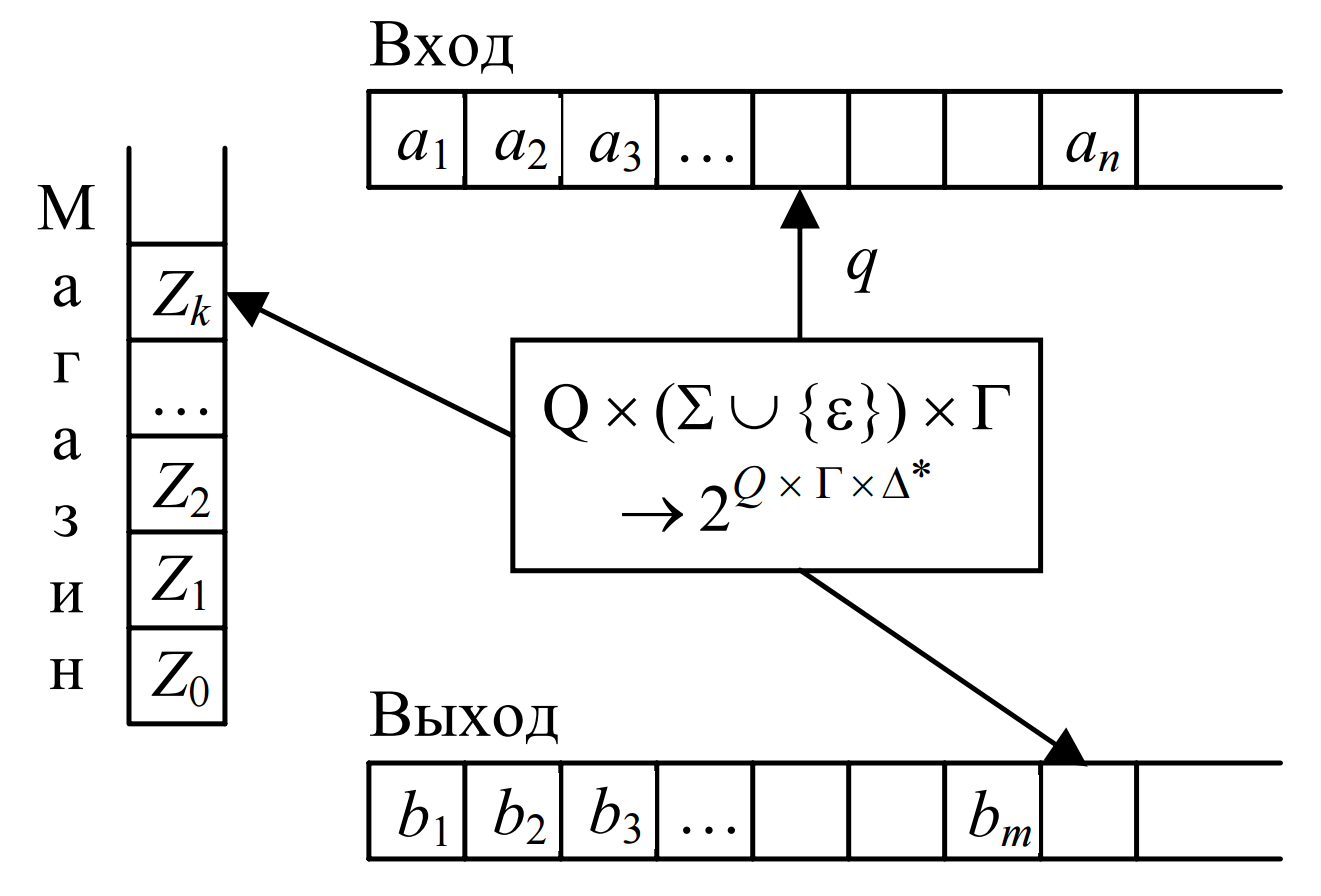
\includegraphics[width=\textwidth]{pics/transducer.png}
\end{center}

\end{frame}

\begin{frame}[fragile]
  \transwipe[direction=90]
  \frametitle{Что такое магазинный преобразователь: неформально}
 \begin{center}
    Магазинный автомат, который при каждом переходе пишет что-то в выходную строку
 \end{center}
\end{frame}


\begin{frame}[fragile]
  \transwipe[direction=90]
  \frametitle{Формальное определение}

  \begin{center}
    Магазинный преобразователь это набор $(Q, \Sigma, \Gamma, \Delta, \delta, q_0, Z_0, F)$
  \end{center}
  \begin{itemize}
    \item $Q$ --- конечное множество состояний
    \item $\Sigma$ --- конечное множество символов, входной алфавит
    \item $\Gamma$ --- конечное множество символов, стековый алфавит
    \item $\Delta$ --- конечное множество символов, выходной алфавит
    \item $\delta \subseteq Q \times (Z \cup \varepsilon) \times \Gamma \rightarrow 2^{Q \times \Gamma^* \times \Delta^*}$ --- отношение переходов
    \item $q_0 \in Q$ --- стартовое состояние
    \item $Z_0 \in \Gamma$ --- начальный элемент стека
    \item $F \subseteq Q$ --- множество принимающих (конечных) состояний
  \end{itemize}
\end{frame}

\begin{frame}[fragile]
  \transwipe[direction=90]

\begin{center}
    \frametitle{Отношение переходов}
    $\delta(p, a, Z) = \{(q_i, \gamma_i, \alpha_i) \, | \, 1 \leq i \leq n \}$  означает
\end{center}

  \begin{itemize}
    \item Если магазинный преобразователь находится в состоянии $p \in Q$, на вершине стека находится $Z \in \Gamma$, а со входа читается символ $a \in \Sigma \cup \varepsilon$, то для некоторого $i$:
    \begin{itemize}
      \item Изменяем состояние на $q_i \in Q$
      \item Снимаем со стека символ $Z$, записываем на стек строку $\gamma_i \in \Gamma^*$
      \item В выходную строку дописываем $\alpha_i \in \Delta^*$
    \end{itemize}
    \item $\Sigma \cup \varepsilon$ сигнализирует о том, что вход можно и не читать
    \item Если $\gamma_i = \varepsilon$, символ со стека стирается
    \item Если $\alpha_i = \varepsilon$, в выходную строку ничего не пишем
  \end{itemize}
\end{frame}

\begin{frame}[fragile]
  \transwipe[direction=90]
  \frametitle{Семантика магазинного преобразователя}
\begin{itemize}
  \item Мгновенное описание МП: $(p, \omega, \beta, \alpha) \in Q \times \Sigma^* \times \Gamma^* \times \Delta^*$
  \begin{itemize}
    \item $p$ --- текущее состояние автомата
    \item $\omega$ --- непрочитанный фрагмент входного потока
    \item $\beta$ --- содержимое стека (верхушка записана первой)
    \item $\alpha$ --- содержимое выходной ленты
  \end{itemize}
  \item Отношение $\vdash$ на мгновенных описаниях (шаг)
  \begin{itemize}
    \item Для каждого $(q, \gamma, \alpha) \in \delta(p, a, Z)$, верно $(p, a x, Z \eta, \zeta) \vdash (q, x, \gamma \eta, \alpha \zeta)$ для произвольных $x \in \Sigma^*, \eta \in \Gamma^*, \zeta \in \Delta^*$
  \end{itemize}
  \item Шаг не определен, если стек пуст
\end{itemize}

\end{frame}

\begin{frame}[fragile]
  \transwipe[direction=90]
  \frametitle{Семантика магазинного преобразователя: вычисление}
  \begin{itemize}
    \item Вычисление  --- последовательность шагов
    \begin{itemize}
      \item $\vdash^*$ --- транизитивно рефлексивное замыкание отношения $\vdash$
    \end{itemize}
    \item Начальное мгновенное описание $(q_0, \omega, Z_0, \varepsilon)$
    \item Два варианта окончания работы
    \begin{itemize}
      \item По достижении конечного состояния
      \begin{itemize}
        \item $\tau(M) = \{ (\omega, \alpha) \, | \, \omega \in  \Sigma^*, \alpha \in \Delta^*, (q_0, \omega, Z_0, \varepsilon) \vdash^* (f, \varepsilon, \gamma, \alpha),$

        $\ \ \ \ \ \ \ \ \ \ \ \ \ \ \ \ \ \ \ \ \ \ f \in F, \gamma \in \Gamma^* \}$
      \end{itemize}
      \item По опустошении стека
      \begin{itemize}
        \item $\tau_{\varepsilon}(M) = \{ (\omega, \alpha) \, | \, \omega \in  \Sigma^*, \alpha \in \Delta^*, (q_0, \omega, Z_0, \varepsilon) \vdash^* (q, \varepsilon, \varepsilon, \alpha), q \in Q\}$
      \end{itemize}
      \item Эти варианты эквивалентны: по преобразователю, завершающемуся по первой схеме, можно посмотроить преобразователь, завершающийся по второй схеме, и наоборот
    \end{itemize}

  \end{itemize}
\end{frame}

\begin{frame}[fragile]
  \transwipe[direction=90]
  \frametitle{Детерминированные магазинные преобразователи}
\begin{center}
    Магазинный преобразователь является \textbf{детерминированным}, если
\end{center}

\begin{itemize}
  \item $\forall q \in Q, a \in \Sigma \cup \{ \varepsilon \}, Z \in \Gamma:  | \delta(q, a, Z) | \leq 1$
  \item Если $ \delta(q, \varepsilon, Z) \neq \varnothing$, то $\forall a \in \Sigma: \delta(q, a, Z) = \varnothing$
  \item Детерминированный магазинный преобразователь является частным случаем недетерминированного
\end{itemize}
\end{frame}

\begin{frame}[fragile]
  \transwipe[direction=90]
  \frametitle{Пример: преобразование префиксных арифметических выражений в постфиксные}
$$M = \{ \{ q \}, \{ a, +, * \}, \{ E, +, * \}, \{ a, +, * \}, \delta, q, E, \{ q \} \}$$

$$
\begin{array}{crcl}
&\delta(q, a, E)& = & \{ (q, \varepsilon, a) \} \\
&\delta(q, +, E)& = & \{ (q, EE+, \varepsilon) \} \\
&\delta(q, *, E)& = & \{ (q, EE*, \varepsilon) \} \\
&\delta(q, \varepsilon, +)& = & \{ (q, \varepsilon, +) \} \\
&\delta(q, \varepsilon, *)& = & \{ (q, \varepsilon, *) \}
\end{array}
$$

\vfill

$(q, +*aaa, E, \varepsilon) \vdash (q, *aaa, EE+, \varepsilon) \vdash (q, aaa, EE*E+, \varepsilon) \vdash (q, aa, E*E+, a) \vdash (q, a, *E+, aa) \vdash (q, a, E+, aa*) \vdash (q, \varepsilon, +, aa*a) \vdash (q, \varepsilon, \varepsilon, aa*a+)$
\end{frame}

\begin{frame}[fragile]
  \transwipe[direction=90]
  \frametitle{Взаимоотношение между простыми СУ-схемами и магазинными преобразователями}
  \begin{rutheorem}[]
    По простой СУ-схеме $( N, \Sigma, \Delta, R, S )$  можно построить магазинный преобразователь, задающий эквивалентную трансляцию
  \end{rutheorem}

  \vfill

  \begin{rutheorem}[]
    По магазинному преобразователю $P = (Q, \Sigma, \Gamma, \Delta, \delta, q_0, Z_0, \varnothing) $ можно построить простую СУ-схему, задающую эквивалентную трансляцию
  \end{rutheorem}

  \vfill

  \begin{rutheorem}[]
    Класс трансляций, задаваемых простыми СУ-трансляциями совпадает с классом трансляций, задаваемых магазинными автоматами
  \end{rutheorem}
\end{frame}


\begin{frame}[fragile]
  \transwipe[direction=90]
  \frametitle{Однозначные СУ-схемы и левосторонний вывод}



\begin{rutheorem}[]
Выходная цепочка однозначной СУ-схемы может быть сгенерирована при левостороннем выводе входной цепочки
\end{rutheorem}

\end{frame}



\begin{frame}[fragile]
  \transwipe[direction=90]
  \frametitle{Транслирующие грамматики}
  \begin{itemize}
    \item КС-грамматика, терминальный алфавит которой разбит на два множества: входных и выходных символов
    \item \textbf{Транслирующая грамматика} --- пятерка $(N, \Sigma_i, \Sigma_o, P, S)$
    \begin{itemize}
      \item $N$ --- алфавит нетерминалов
      \item $\Sigma_i$ --- алфавит входных терминалов
      \item $\Sigma_o$ --- алфавит выходных терминалов
      \item $S \in N$ --- стартовый нетерминал
      \item $P = \{ A \rightarrow \alpha \}, \alpha \in (\Sigma_i \cup \Sigma_o \cup N)^*$ --- множество правил вывода
    \end{itemize}
  \end{itemize}
\end{frame}

\begin{frame}[fragile]
  \transwipe[direction=90]
  \frametitle{Пример транслирующей грамматики}
$$
\begin{array}{cccl}
&E& \rightarrow & E + T \, \{ + \} \\
& &    |        & T   \\
&T& \rightarrow & T * F \, \{ * \} \\
& &    |        & F  \\
&F& \rightarrow & n \, \{ n \} \\
& &    |        & ( E ) \\
\end{array}
$$
\pause ~\\~

$E \derives E + T \, \{ + \} \derives T + T \, \{ + \} \derives F + T \, \{ + \} \derives n \, \{ n \} + T \, \{ + \} \derives n \, \{ n \} + T * F \, \{ * \} \, \{ + \} \derives n \, \{ n \} + F * F \, \{ * \} \, \{ + \} \derives n \, \{ n \} +  n \, \{ n \} * F \, \{ * \} \, \{ + \} \derives n \, \{ n \} +  n \, \{ n \} * n \, \{ n \} \, \{ * \} \, \{ + \}$

\pause
\begin{itemize}
  \item Если вычеркнуть все выходные символы, получим $n + n * n$
  \item Если вычеркнуть все входные символы, получим $n \, n \, n + *$ --- постфиксная запись выражения
\end{itemize}
\end{frame}


\begin{frame}[fragile]
  \transwipe[direction=90]
  \frametitle{Постфиксная транслирующая грамматика}
  \begin{itemize}
    \item Если выходные символы встречаются только в конце правил, транслирующая грамматика называется постфиксной
    \item Это требование формально не выдвигается: транслирующие грамматики могут быть не постфиксными
    \item На практике постфиксные транслирующие грамматики удобнее
  \end{itemize}
\end{frame}

\begin{frame}[fragile]
  \transwipe[direction=90]
  \frametitle{Атрибутная транслирующая грамматика}
  \begin{itemize}
    \item Входной алфавит --- алфавит лексем
    \begin{itemize}
      \item Лексема характеризуется \textbf{типом} и \textbf{значением}
    \end{itemize}
    \item Транслирующая грамматика описывает перевод только \textbf{типа} лексемы
    \begin{itemize}
      \item Это существенно снижает выразительность формализма
    \end{itemize}
    \item Для борьбы с этим недостатком предложены атрибутные грамматики
    \begin{itemize}
      \item Модификация транслирующих грамматик, снабженная атрибутами
      %\item Выходные символы транслирующих грамматик --- транслирующие символы
      %\begin{itemize}
      %  \item Нетерминалы, которые раскрываются в $\varepsilon$, и в момент раскрытия выполняют связанные с ними действие
      %\end{itemize}
    \end{itemize}
  \end{itemize}
\end{frame}


\begin{frame}[fragile]
  \transwipe[direction=90]
  \frametitle{Атрибут}

\begin{center}
    \textbf{Атрибут} --- дополнительные данные, ассоциированные с грамматическими символами
\end{center}
  \begin{itemize}
    \item Если $X$ --- символ, а $a$ --- его атрибут, то значение $a$ в узле дерева, помеченном $X$, записывается как $X.a$
    \item Узлы дерева могут реализовываться как записи или объекты, а атрибуты --- как поля
    \item Атрибуты могут быть любого типа
    \item Если в каждом узле дерева атрибуты уже вычислены, оно называется \textbf{аннотированным}
    \item Процесс вычисления этих атрибутов называется \textbf{аннотированием} дерева разбора
  \end{itemize}
\end{frame}

\begin{frame}[fragile]
  \transwipe[direction=90]
  \frametitle{Вычисление атрибутов не всегда возможно}
$$
\begin{array}{clcl}
&A \rightarrow    B   & & A.s = B.i \\
&                     & & B.i = A.s + 1
\end{array}
$$
\end{frame}


\begin{frame}[fragile]
  \transwipe[direction=90]
  \frametitle{Синтезируемый атрибут, S-атрибутная грамматика}
  \begin{itemize}
    \item Атрибут, значение которого зависит от значений атрибутов детей данного узла или от других атрибутов этого узла, называется \textbf{синтезируемым}
    \item Если в транслирующей грамматике используются только синтезируемые атрибуты, она называется \textbf{S-атрибутной грамматикой}
    \item Аннотирование дерева разбора S-атрибутной грамматики возможно путем выполнения семантических правил снизу вверх (от листьев к корню)
  \end{itemize}

\end{frame}


\begin{frame}[fragile]
  \transwipe[direction=90]
  \frametitle{Пример S-атрибутной грамматики}
$$
\begin{array}{ccclll}
&S  & \rightarrow & E       &                                &\{S.val = E.val\}\\~\\

&E^0& \rightarrow & E^1 + T &                                &\{E^0.val = E^1.val + T.val\}\\~\\

&E  & \rightarrow & T       &                                &\{E.val = T.val\}\\~\\

&T^0& \rightarrow & T^1 * F &                                &\{T^0.val = T^1.val * F.val\}\\~\\

&T  & \rightarrow & F       &                                &\{T.val = F.val\}\\
&F  & \rightarrow & n       &                                &\{F.val = n.val\}\\
&F  & \rightarrow & (E)     &                                &\{F.val = E.val\}\\

\end{array}
$$
\end{frame}

\begin{frame}[fragile]
  \transwipe[direction=90]
  \frametitle{Наследуемый атрибут, L-атрибутная грамматика}
Атрибут, значение которого зависит только от атрибутов братьев узла слева или атрибутов родителей, называется \textbf{наследуемым}

\vfill

Грамматика называется \textbf{L-атрибутной}, если каждый наследуемый
атрибут узла $X_j$ в правиле $A \to X_1 \dots X_n$ зависит только от:

\begin{itemize}
  \item Атрибутов узлов $X_1 \dots X_{j-1}$ (братья слева)
  \item Наследуемых атрибутов узла $А$ (предок)
\end{itemize}

\vfill

Синтезируемые атрибуты тоже разрешены

\vfill

Любая S-атрибутная грамматика является L-атрибутной
\end{frame}

\begin{frame}[fragile]
  \transwipe[direction=90]
  \frametitle{Пример L-атрибутной грамматики}
$$
\begin{array}{ccclll}
&D  & \rightarrow & TL      &                                &\{L.inh = T.type;\\
&   &             &         &                                &  D.val = L.val\} \\
&T  & \rightarrow & int     &                                &\{T.type = integer\}\\
&T  & \rightarrow & real    &                                &\{T.type = real\}\\~\\

&L^0& \rightarrow & L^1, id &                                &\{L^1.inh = L^0.inh\}\\
&   &             &         &                                &\{L^0.val = (id.text, L_0.inh) :: L^1.val\}\\~\\

& L & \rightarrow &  id     &                                &\{[id.text, L.inh]\}\\
\end{array}
$$
\end{frame}

\end{document}
